\begin{figure}[h] 
\centering 
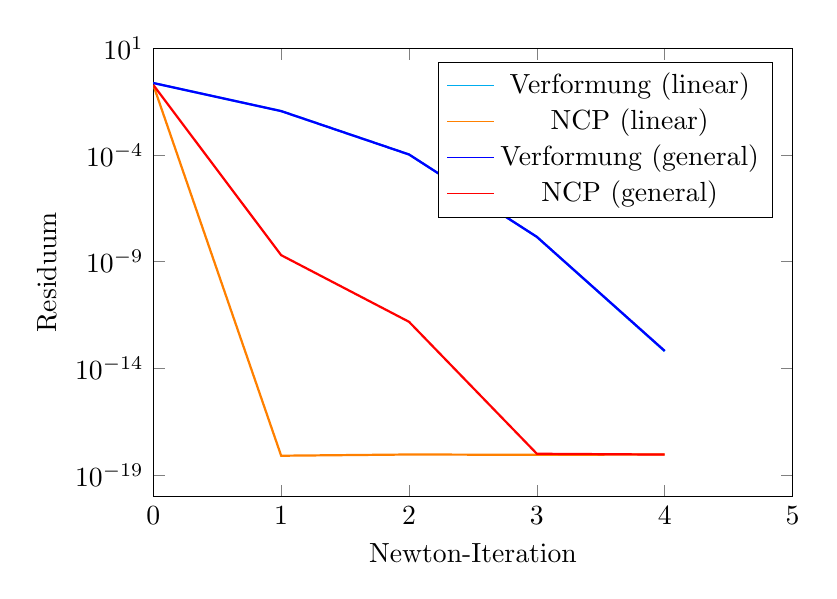
\begin{tikzpicture}[every plot/.append style={thick}] 
\begin{axis}[ 
label style={font=\normalsize}, 
xlabel={Newton-Iteration}, 
ylabel={Residuum}, 
xmin=0, xmax=5, 
ymode=log, 
ymin=0, ymax=10, 
width=0.8\textwidth, 
height=0.6\textwidth, 
legend pos=north east, 
legend style={cells={align=left}}, 
grid style=dashed, 
] 
\addplot[ 
color=cyan, 
] 
coordinates { 
(0, 2.33e-01)(1, 1.13e-02)(2, 1.05e-04)(3, 1.45e-08)(4, 6.41e-14)}; 
\addlegendentry{Verformung (linear)} 
\addplot[ 
color=orange, 
] 
coordinates { 
(0, 1.88e-01)(1, 8.17e-19)(2, 9.32e-19)(3, 9.02e-19)(4, 9.33e-19)}; 
\addlegendentry{NCP (linear)} 
\addplot[ 
color=blue, 
] 
coordinates { 
(0, 2.33e-01)(1, 1.13e-02)(2, 1.05e-04)(3, 1.45e-08)(4, 6.63e-14)}; 
\addlegendentry{Verformung (general)} 
\addplot[ 
color=red, 
] 
coordinates { 
(0, 1.90e-01)(1, 2.02e-09)(2, 1.53e-12)(3, 1.01e-18)(4, 9.26e-19)}; 
\addlegendentry{NCP (general)} 
\end{axis} 
\end{tikzpicture} 
\caption{Residuen des Stoffgesetzes 'Neo Hooke' mit Hinderniss 'Parabel' und 33282 Freiheitsgraden für die Verschiebung.} 
\label{fiq:NeoHooke_Parabel_level6} 
\end{figure} 
